\chapter{INTRODUCTION}
\label{chap:introduction}

\section{Jaguar Conservation}

The jaguar (Panthera onca) is the largest neotropical felid and a keystone apex predator. Historically distributed from the southern United States to Argentine Patagonia the jaguar now occupies only about 46\% of its original range, with an estimated 173,000 individuals remaining—roughly half in Brazil \cite{jedrzejewski2018estimating}. Jaguars inhabit diverse ecosystems, from dense tropical forests to wetlands, and their protection benefits numerous other species, making them an umbrella species for biodiversity conservation.

Population status varies greatly across biomes. The Amazon and Pantanal harbor the largest, most genetically diverse populations, with extensive connectivity and high habitat suitability. In contrast, the Atlantic Forest and Caatinga populations are small, isolated, and genetically impoverished due to severe fragmentation, while the Cerrado has seen a decline exceeding 50\% \cite{haag2010effect}. Connectivity corridors, such as along the Araguaia and Paraguay Rivers, are critical to maintain gene flow and avoid local extinctions.

Habitat loss and fragmentation remain the most severe threats. While habitat loss reduces total area, fragmentation more acutely undermines survival by isolating populations and limiting dispersal, especially in smaller groups. In Brazil, most jaguars now occur in protected areas, yet many of these are too small or disconnected to ensure long-term viability. Only in the Amazon do some reserves have sufficient size for multi-century persistence, underscoring the need for connected protected areas and carefully planned dispersal corridors \cite{rabinowitz2010long}.

\begin{figure}[H]
\centering
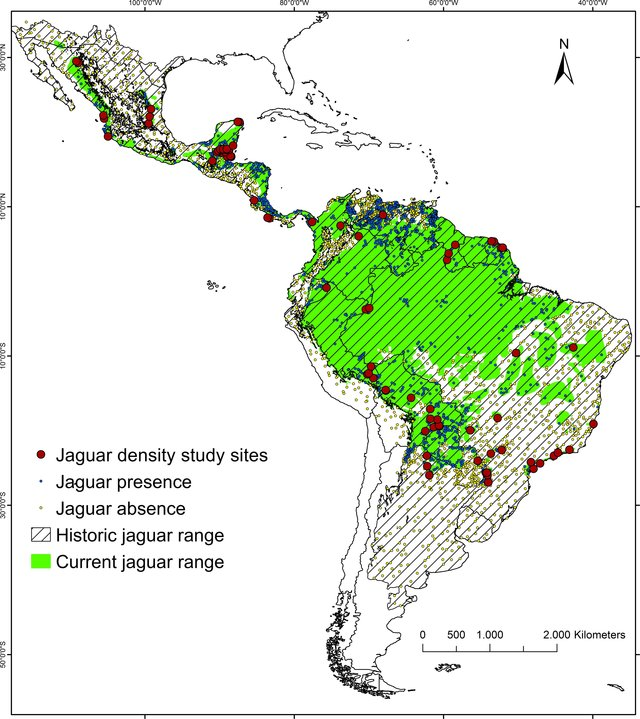
\includegraphics[width=0.7\textwidth]{images/image5.png}
\caption{Historical (light shading) and current (dark shading) distribution of the jaguar (\textit{Panthera onca}) across the Americas. Data adapted from \cite{jedrzejewski2018estimating}.}
\label{fig:jaguar_distribution}
\end{figure}

Human-wildlife conflict and illegal trade compound these pressures. Retaliatory killing is common where jaguars prey on livestock, and a growing black market, driven largely by demand from Asian countries for skins, teeth, and bones, targets populations across the Amazon and beyond \cite{morcatty2020illegal}. Enforcement is hampered by weak governance, legal loopholes, and clandestine trafficking networks.

A critical gap in conservation is the ability to assign poached individuals to their population of origin, which would allow authorities to identify and prioritize anti-poaching interventions at key hunting hotspots. Strengthening governance, enhancing forensic tools for geographic assignment, expanding protected habitats, and disrupting trafficking routes are therefore essential for the long-term survival of the species.

\section{Conservation Genomics and Machine Learning}

A wide range of disciplines is involved in biodiversity conservation and ecosystem services. Traditionally, genetics has helped elucidate how evolutionary processes shape genotypic and phenotypic variation and determine the population structure of a species, in addition to identifying potential risks related to demographic change and inbreeding on population viability. With the advancement of genetic technology, another new field emerged, genomics, which brought a dramatic increase in the number of genetic markers that should improve the accuracy of diversity estimates and demographic parameters of populations relevant to conservation \cite{shafer2015genomics}.

Among the greatest contributions of genomics to conservation is the ability to predict extinction risks and inform managers about population viability before population decline, allowing decisions on whether translocation is a viable strategy, through the identification of loci and genomic regions responsible for adaptation to local conditions \cite{mcmahon2014how}. Population size is also a key factor in determining demographic viability, and this can be estimated through marker panels designed for individual identification and kinship relationships \cite{hohenlohe2021population}. Another area where genomic data is particularly useful and classical genetic techniques are insufficient is the study of past population dynamics of an endangered species – this allows us to elucidate whether the species suffered declines during its past evolutionary history or if its current status is a consequence of what is currently happening.

Machine learning (ML) is increasingly being integrated into conservation genomics to address complex, high-dimensional datasets. ML models can classify individuals into populations of origin, detect cryptic population structures, and predict adaptive traits by learning patterns across thousands or millions of genomic markers.

In addition, ML methods can be used to detect signals of selection, predict future population trends under different environmental scenarios, and integrate genomic, environmental, and movement data for more precise conservation planning. For example, combining genomic data with remote sensing and ecological variables in predictive models can help identify climate-resilient habitats and forecast range shifts. Similarly, unsupervised learning techniques such as clustering and dimensionality reduction can reveal hidden genetic structures that may not be apparent with traditional methods, guiding the design of protected areas and connectivity corridors.

\section{The Challenge of Limited Data in Endangered Species}

A critical challenge in conservation genomics is the limited availability of genetic data for endangered species. This scarcity stems from several factors: small population sizes, difficulties in sample collection, ethical considerations, and the high cost of genomic sequencing. Traditional approaches to geographic assignment and population structure analysis often require substantial datasets to achieve reliable results, creating a paradox where the species most in need of conservation attention have the least data available for analysis.

This limitation is particularly acute for jaguars, where population fragmentation and small sample sizes in critical regions (such as the Atlantic Forest) make it difficult to develop robust models for geographic assignment. While SNP-based approaches have provided valuable insights, they often require large numbers of individuals per population to achieve sufficient precision, especially when dealing with subtle genetic differentiation between recently fragmented populations \cite{lazzari2025development, haag2010effect}.

\section{The Promise of Transfer Learning in Conservation Genomics}

Recent advances in machine learning, particularly in the field of natural language processing, have introduced powerful techniques for learning from limited data through transfer learning. These approaches allow models pre-trained on large, general datasets to be fine-tuned for specific tasks with much smaller datasets, often achieving superior performance compared to models trained from scratch.

In the context of genomics, foundation models like DNABERT-2 \cite{zhou2024dnabert} have demonstrated remarkable capabilities in understanding DNA sequence patterns across multiple species. These models can capture complex genomic features and relationships that may not be apparent through traditional analytical methods. By leveraging the knowledge learned from large, diverse genomic datasets, these models can potentially overcome the data scarcity challenges faced in endangered species conservation.
